\newpage

\section{Постановка задачи}

Задан временной ряд 
$$x_{0}, x_{1}, x_{2}, ... x_{N}, \quad x_{i} \in \mathbb{R}^{6}$$
$$
    x_{i} &= 
    \begin{bmatrix}
        c_{i} & o_{i} & h_{i} & l_{i} & a_{i}
    \end{bmatrix}^{T},
$$
где \\
$c_{i}$ - цена закрытия, \\
$o_{i}$ - цена открытия, \\
$h_{i}$ - максимальная цена, \\
$l_{i}$ - минимальная цена, \\
$a_{i}$ - ответ модели автоследования ($a_{i} = 0$ в базовом варианте обучения модели)

\subsection{Постановка задача прогнозирования}

Требуется получить модель временного ряда:
$$\hat{c}_{t+k}(\mathbf{w}) = f_{t,k}(x_{t-M}, ..., x_{t}; \mathbf{w})$$
$$k = 1, ..., K,$$
где  \\
$K$ - горизонт прогнозирования, \\
$M$ - количество предыдущих наблюдений, \\
$\mathbf{w}$ - вектор параметров модели.

С помощью скользящего окна составлена выборка $\mathfrak{D}=(\mathbf{X},\mathbf{Y})$:

\begin{figure}[h!t]\center
{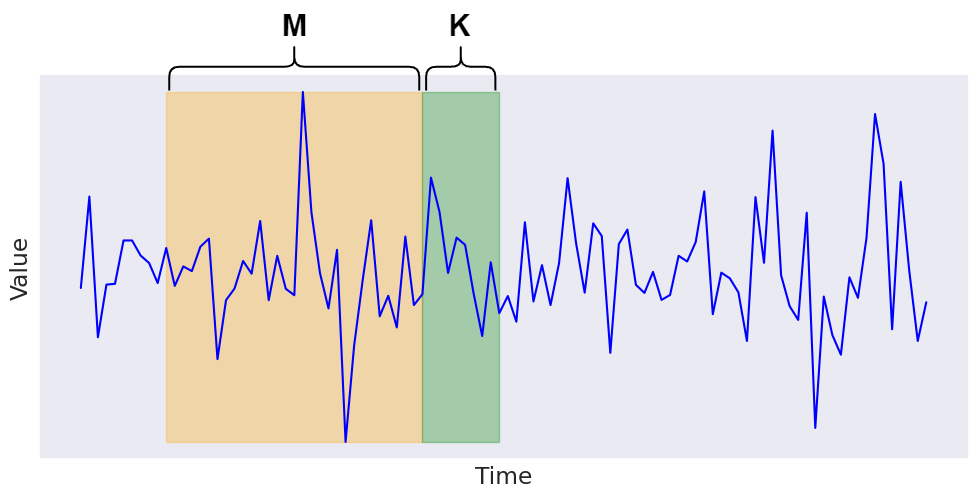
\includegraphics[width=0.8\textwidth]{results/slidingwindow.png}}
\caption{Использование скользящего окна для составления выборки}
\end{figure}

$
\mathbf{X} = \begin{pmatrix}
x_{0} & x_{1} & x_{2} & ... & x_{M}\\
x_{1} & x_{2} & x_{3} & ... & x_{M+1} \\
x_{2} & x_{3} & x_{4} & ... & x_{M+2} \\
\vdots & \vdots & \vdots & \vdots & \vdots \\
x_{N-K-M} & x_{N-K-M+1} & x_{N-K-M+2} & ... & x_{N-K} \\
\end{pmatrix} 

\mathbf{Y} = \begin{pmatrix}
c_{M+1} & c_{M+2} & c_{M+3} & ... & c_{M+K}\\
c_{M+2} & c_{M+3} & c_{M+4} & ... & c_{M+K+1} \\
c_{M+3} & c_{M+4} & c_{M+5} & ... & c_{M+K+2} \\
\vdots & \vdots & \vdots & \vdots & \vdots \\
c_{N-K+1} & c_{N-K+2} & c_{N-K+3} & ... & c_{N} \\
\end{pmatrix}
$

Функция потерь $\mathcal{L}$, используемая при обучении модели:
\[
\begin{aligned}
    \mathcal{L}(\mathbf{w,X,Y}) =& \sum\limits_{i=1}^{m}(f_{t,k}(x_{t-M}, ..., x_{t}; \mathbf{w})-c_{t+k}),
\end{aligned}
\]

Получаем оптимизационную задачу:
$$\hat{\mathbf{w}} = \arg\min_{\mathbf{w} \in \mathbb{W}} \mathcal{L}(\mathbf{w,X,Y,f}).$$